\begin{task}{66}
Планарен ли следующий граф? Если да, то нарисуйте его без самопересечений, если нет, то найдите в нём подграф, гомеоморфный $K_{3,3}$.
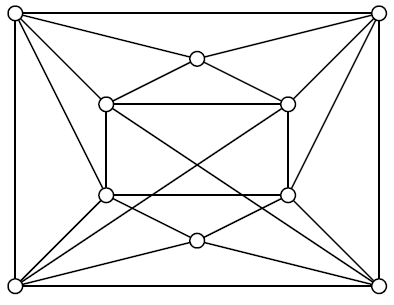
\includegraphics[width = 150pt]{img/id66.png}
\end{task}

\begin{solution}
Занумеруем вершины графа и выделим в нем подграф $K_{3,3}$ (отмечен на рисунке).

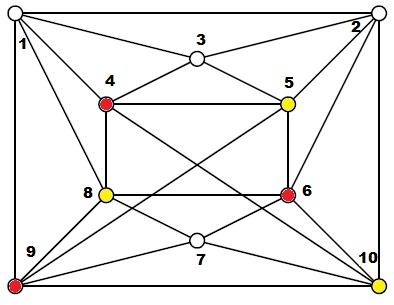
\includegraphics[width = 350pt]{img/id66_final.jpg}.

Так как граф $K_{3,3}$ гомеоморфен самому себе, то по критерию Понтрягина-Куратовского исходный граф не планарен.
\end{solution}